
\section{Derivable functions can be described in first-order logic}
\label{sec:to-logic}
The goal of this section is to show the right-to-left implication of Theorem~\ref{thm:main}, which says that derivable functions can be implemented by first-order transductions. 

As discussed in the body of the paper, we proceed by induction on the derivation. During this induction, we will need to show that every prime function is a first-order transduction. Prime functions are not tree-to-tree functions, instead they transform dataypes into datatypes. This is the reason why we need 
\begin{itemize}
\item to generalize tree-to-tree transductions into  transductions that can transform models over arbitrary vocabularies (and not only the vocabulary of trees). 
\item show how datatypes (terms, pairs, copairs and folds) can be encoded as models over a well chosen vocabulary. More precisely, we will associate to every datatype $\rSigma$ a relational vocabulary that we call \emph{vocabulary of $\rSigma$}. Structures over this vocabulary will be called \emph{models over $\rSigma$}. Then we will define a function
\begin{align*}
    \xymatrix@C=2cm{
        \rSigma \ar[r]^-{x \mapsto \underline x} &
 \text{models over $\rSigma$}
    }
\end{align*} 
which assigns to each element $x \in \rSigma$ a corresponding model  over $\rSigma$, which is denoted by $\underline x$.
\end{itemize}
 
 Right-to-left implication of Theorem~\ref{thm:main} can be then generalized to the following statement, more suited to a proof by induction:

\begin{proposition}\label{prop:main-right-to-left}
Let $\rGamma$ and $\rSigma$ be two datatype.  For every derivable function $\ranked{f}$, there is a first-order transduction $g$ such that the following diagram commutes
  \begin{align*}
  \xymatrix@C=2.8cm{
          \rSigma 
        \ar[d]_{x \mapsto \underline x}
        \ar[r]^-{\ranked{f}}
        &
    \rGamma \ar[d]^{x \mapsto \underline x}
        \\
      \text{models over $\rSigma$}
        \ar[r]_-{g}
        &
    \text{models over $\rGamma$}   
    } 
\end{align*}  
\end{proposition}

The rest of this section is organized as follows. We define first-order transductions transforming arbitrary models in Section~\ref{sec:fo-transduction-def}. In Section~\ref{sec:data-as-models} we define the vocabularies for the  datatypes and the model representation $x \mapsto \underline x$. Finally, we prove Proposition~\ref{prop:main-right-to-left} which gives as a corollary the right-to-left implication of Theorem~\ref{thm:main}.

\subsection{First-order transductions}\label{sec:fo-transduction-def}
The following definition introduces first-order transductions, which generalizes tree-to-tree transductions given in Definition~\ref{def:fo-transduction} to arbitrary models.  

\begin{definition}[First-order transduction]\label{def:fo-transduction-gen}\ 
    A \emph{first-order transduction} is defined to be any  composition of the following two kinds of transformations on structures:
\begin{enumerate}
    \item \emph{Copying.} Fix some  relational vocabulary $\ranked \sigma$ and let $k \in \set{1,2,\ldots}$. Define $k$-copying to be the operation of type 
    \begin{align*}
    \xymatrix{
     \text{models over $\ranked \sigma$} \ar[d]\\
     \txt{models over $\ranked \sigma$  extended\\
with a $k$-ary relation $\mathrm{copy}$}
    }
    \end{align*}
which inputs a model $\mathbb A$, and outputs $k$ disjoint copies of $\mathbb A$, where the  $\mathrm{copy}$ relation is interpreted as the set of tuples $(a_1,\ldots,a_k)$ such that, for  some $a \in \mathbb A$, the first copy of $a$ is  $a_1$, the second copy of $a$ is $a_2$, etc. The $\mathrm{copy}$ relation  is not commutative, because we distinguish the copies.
\item    \emph{Non-copying first-order transduction.} The syntax of a \emph{non-copying first-order transduction}  is given by:
\begin{enumerate}
    \item Input relational vocabulary $\ranked\sigma$ and output relational vocalbulary $\ranked{\gamma}$.
    \item A first-order \emph{universe formula} $\varphi(x)$ over $\ranked{\sigma}$.
    \item For every relation $R$ in vacubulary $\ranked{\gamma}$, a first-order  formula $\varphi_R(x_1,\ldots,x_{\arity R})$ over $\ranked{\sigma}$.
\end{enumerate}
The semantics of a non-copying first-order transduction is  a function
\begin{align*}
    \xymatrix{
        \text{models over $\ranked \sigma$} \ar[d]\\
        \text{models over $\ranked \gamma$}
    }
\end{align*}
defined as follows. If the input model is $\mathbb A$, then the output model is defined as follows: the universe is elements of $\mathbb A$ which satisfy the universe formula, and each relation $R$ is interpreted as those tuples that satisfy $\varphi_R$. 
 \end{enumerate}
\end{definition}

The notion of copying used in the above definition is slightly different from the notion of copying used for tree-to-tree transductions in Definition~\ref{def:fo-transduction}, which was specifically tailored to stay within the realm of trees. Nevertheless, the two definitions are easily seen to define the same class of tree-to-tree functions.
 
\subsection{Datatypes  as models.}\label{sec:data-as-models}
Let us show how to encode datatypes as relational vocabularies and data as models over these vocabularies. 
\begin{definition}[Associated models for terms, pairs, co-pairs, folds.] \label{def:type-model} To each type  $\rSigma$ we associate a vocabulary, called the \emph{vocabulary of $\rSigma$}, and a map 
    \begin{align*}
        a \in \rSigma \qquad \mapsto \qquad \underbrace{\underline a \in \text{models over the  vocabulary of  $\rSigma$}}_{\text{associated model of $a$}}.
    \end{align*}
    Furthermore, for each $a \in \rSigma$ we  distinguish a  sequence (whose length is the arity of $a$) of elements in $\underline a$, which are called the ports of $\underline a$.   The definitions are by induction on the structure of $\rSigma$, as given below.
    \begin{itemize}
        \item \emph{Finite ranked sets.} Elements of a ranked set   \begin{align*}
        \rSigma =  \set{a_1,\ldots,a_k}
        \end{align*} are modeled  using a vocabulary which has unary relations $a_1,\ldots,a_k$ and $P_1,\ldots,P_m$ where $m$ is the maximal arity of elements in $\rSigma$. 
        For $a \in \rSigma$ of arity $n$, the  universe of $\underline a$ is $\set{0,1,\ldots,n}$, with the ports being $1,\ldots,n$. 
            The  relation $P_i$  is interpreted as $\set i$ when $i \in \set{1,\ldots,n}$ and as the empty set otherwise. The relation $a_i$ is interpreted as $\set 0$ when $a = a_i$ and as the empty set otherwise. 
        \item \emph{Coproduct.}  Elements of the coproduct $\ranked{\Sigma_1 + \Sigma_2}$ are modeled using the disjoint union of the vocabularies of $\ranked{\Sigma_1}$ and $\ranked{\Sigma_2}$. 
            If an element of the coproduct comes from $\ranked{\Sigma_1}$, then its associated model is defined as for the type $\ranked{\Sigma_1}$, with  the remaining relations from the vocabulary of   $\ranked{\Sigma_2}$ interpreted   as empty sets. The definition is analogous for  elements from $\ranked{\Sigma_2}$. 
        \item \emph{Product.}   Pairs in   $\ranked{\Sigma_1 \product \Sigma_2}$ are modeled
        using the disjoint union of the vocabularies of $\ranked{\Sigma_1}$ and $\ranked{\Sigma_2}$. 
            For  $\tensorpair{a_1,a_2}$, the associated model is    the disjoint union of models $\underline{a_1} + \underline {a_2}$, with the relations of $\underline {a_1}$ using the  vocabulary of ${\ranked{\Sigma_1}}$, and the relations of $\underline {a_2}$ using the vocabulary  ${\ranked{\Sigma_1}}$. 
            If $n_1$ is the arity of $a_1$, then the first $n_1$ ports are inherited from  $\underline {a_1}$ and the remaining ports are inherited from  $\underline {a_2}$.
        % \item \emph{Cartesian product.}   Cartesian pairs in  $\ranked{\Sigma_1 \product \Sigma_2}$ are modeled  using the disjoint union of the vocabularies of $\ranked{\Sigma_1}$ and $\ranked{\Sigma_2}$, plus an extra binary relation $R$.  
        %     The model associated to a Cartesian pair   $ (a_1,a_2)$,  is      the disjoint union $\underline{a_1} +  \underline {a_2}$, in the same sense as in the previous item for $\product$,  with the binary relation $R$ interpreted as 
        %         \begin{align*}
        %            \quad \set{(\text{$i$-th port of $\underline {a_1}$}, \text{$i$-th port of $\underline a_2$}): i \in [1,\text{arity of $(a_1,a_2)$}]} 
        %         \end{align*}
        %         The ports are inherited from   $\underline {a_1}$.
        \item \emph{Folding.}   For $k \in \set{1,2,\ldots}$, elements of   $\reduce k \rSigma$ are modeled using the  vocabulary of $\rSigma$ plus two extra binary relations $\portord$ and $R$. If $a \in \rSigma$ has arity $nk$, then the model associated to $a/f$ -- which has arity $n$ --   is obtained from  $\underline{a}$ by adding a copy of the model below, where $\sqsubset$ is the natural ordering on integers
                \begin{align*}
                (\set{1,\ldots,n}, \portord),
                \end{align*}
whose elements are used as the ports, and interpreting the binary relation $R$ as
        \begin{align*}
        \set{(\text{$i$-th port of $\underline a$},f(i)) : i \in \set{1,\ldots,nk}}
        \end{align*}
                
                
        \item \emph{Terms.}   Terms in $\tmonad \rSigma$ are modeled using vocabulary of $\rSigma$ extended with two fresh binary relations $\anceord$ and $\portord$. 
          Let $t \in \tmonad \rSigma$. Consider the disjoint union of models
            \begin{align}\label{eq:non-port}
                 \coprod_{x \in \text{non-port nodes in $t$}} \underline{a(x)},
            \end{align}
         where  $\underline a(x)$ is the model over vocabulary of $\rSigma$ that  is defined by induction assumption.   In the above  disjoint union, the same vocabulary, namely the vocabulary of $\rSigma$,  is used  for all parts of the disjoint union. Next, consider  the model
            \begin{align}\label{eq:ports}
            (\set{1,\ldots,n}, \portord)
            \end{align}
            where $\portord$ is the natural ordering on $\set{1,\ldots,n}$. 
            The model of $t$ is defined by taking the disjoint union of the models in~\eqref{eq:non-port} and~\eqref{eq:ports}, and defining the descendent relation $\anceord$ as the set of pairs $(u,v)$ such that:
            \begin{itemize}
            \item either $u$ is the $i$-th port of $\underline{a(x)}$ for some node $x$ of $a$, $v$ is a port of $\underline{a(y)}$ for some node $y$ which is a descendent of the $i$-th child of $x$.
            \item or $u$ is the $i$-th port of $\underline{a(x)}$ for some node $x$ of $a$, $v=j\in\{1,\dots,n\}$ and the $j$-th port of $a$ is a descendent of the $i$-th child of $x$.
            \end{itemize} 

            % It  consists of all pairs $(u,v)$ such that $u$ is the $i$-th port of $\underline{a(x)}$  some non-port node $x$, and $v$ belongs to $\underline{a(y)}$ for some node (possibly a port) $y$ which is a descendant (not necessarily proper) of the $i$-th child of $x$. The binary relation $\portletter$ is the total order 
           % The ports are taken from the structure~\eqref{eq:ports}.
    \end{itemize}
\end{definition}

The above  definition creates a certain ambiguity for trees, because if $t$ is a tree over a finite ranked set $\rSigma$, then $\underline t$ can be understood in two ways: as per  Definition~\ref{def:tree-model} for trees, or as per Definition~\ref{def:type-model} when $t$ is viewed as a special case of a term $t \in \tmonad \rSigma$. Since we only use first-order transductions to transform relational structures,  this ambiguity is not a problem, because one can easily define first-order transductions which map one definition of $\underline t$ to the other.


\subsection{Proof of Proposition~\ref{prop:main-right-to-left}}
The proof proceeds by induction, following the definition of derivable functions. 
In the induction step, we have to deal with function composition and the lifting of function along the datatype constructors. First-order transductions are closed under composition by definition, while the liftings are immediate. 

In the induction base, we need to show that all of the prime functions are first-order transductions. 
All the cases are easy, and consist mainly on unfolding the definitions; this is the point of calling these functions prime. There is one exception, which requires some more explanation, namely monotone unfolding. We explain below just one of the easy functions, the unit function $\ranked{\Sigma \to \tmonad \Sigma}$, and the monotone unfolding. The other prime functions are left as an exercise. 
    
\subsubsection{A first-order transduction for the term unit}
\label{sec:transduction-unit}
    In the following, it will be convenient to use, as part of the vocabulary of $\rSigma$, a unary relation  $\mathsf{Port}_\rSigma$ which selects the ports of the structures over the vocabulary of $\rSigma$; and a binary relation $\sqsubset_\rSigma$ which orders these ports. By induction on $\rSigma$, we can show that both relations are definable by first-order formulas over  the vocabulary of $\rSigma$.
    
    
   Given an element $x$ of $\rSigma$, let us show how  $\unit(x)$ can be implemented using a first-order transduction.  The copying constant is 2,
    the first copy will contain the whole structure $\underline{x}$ and the second copy will select only the ports of $\underline{x}$ which will serve as the ports of the structure $\underline{\unit(x)}$, as illustrated by the following picture 
\begin{center}
    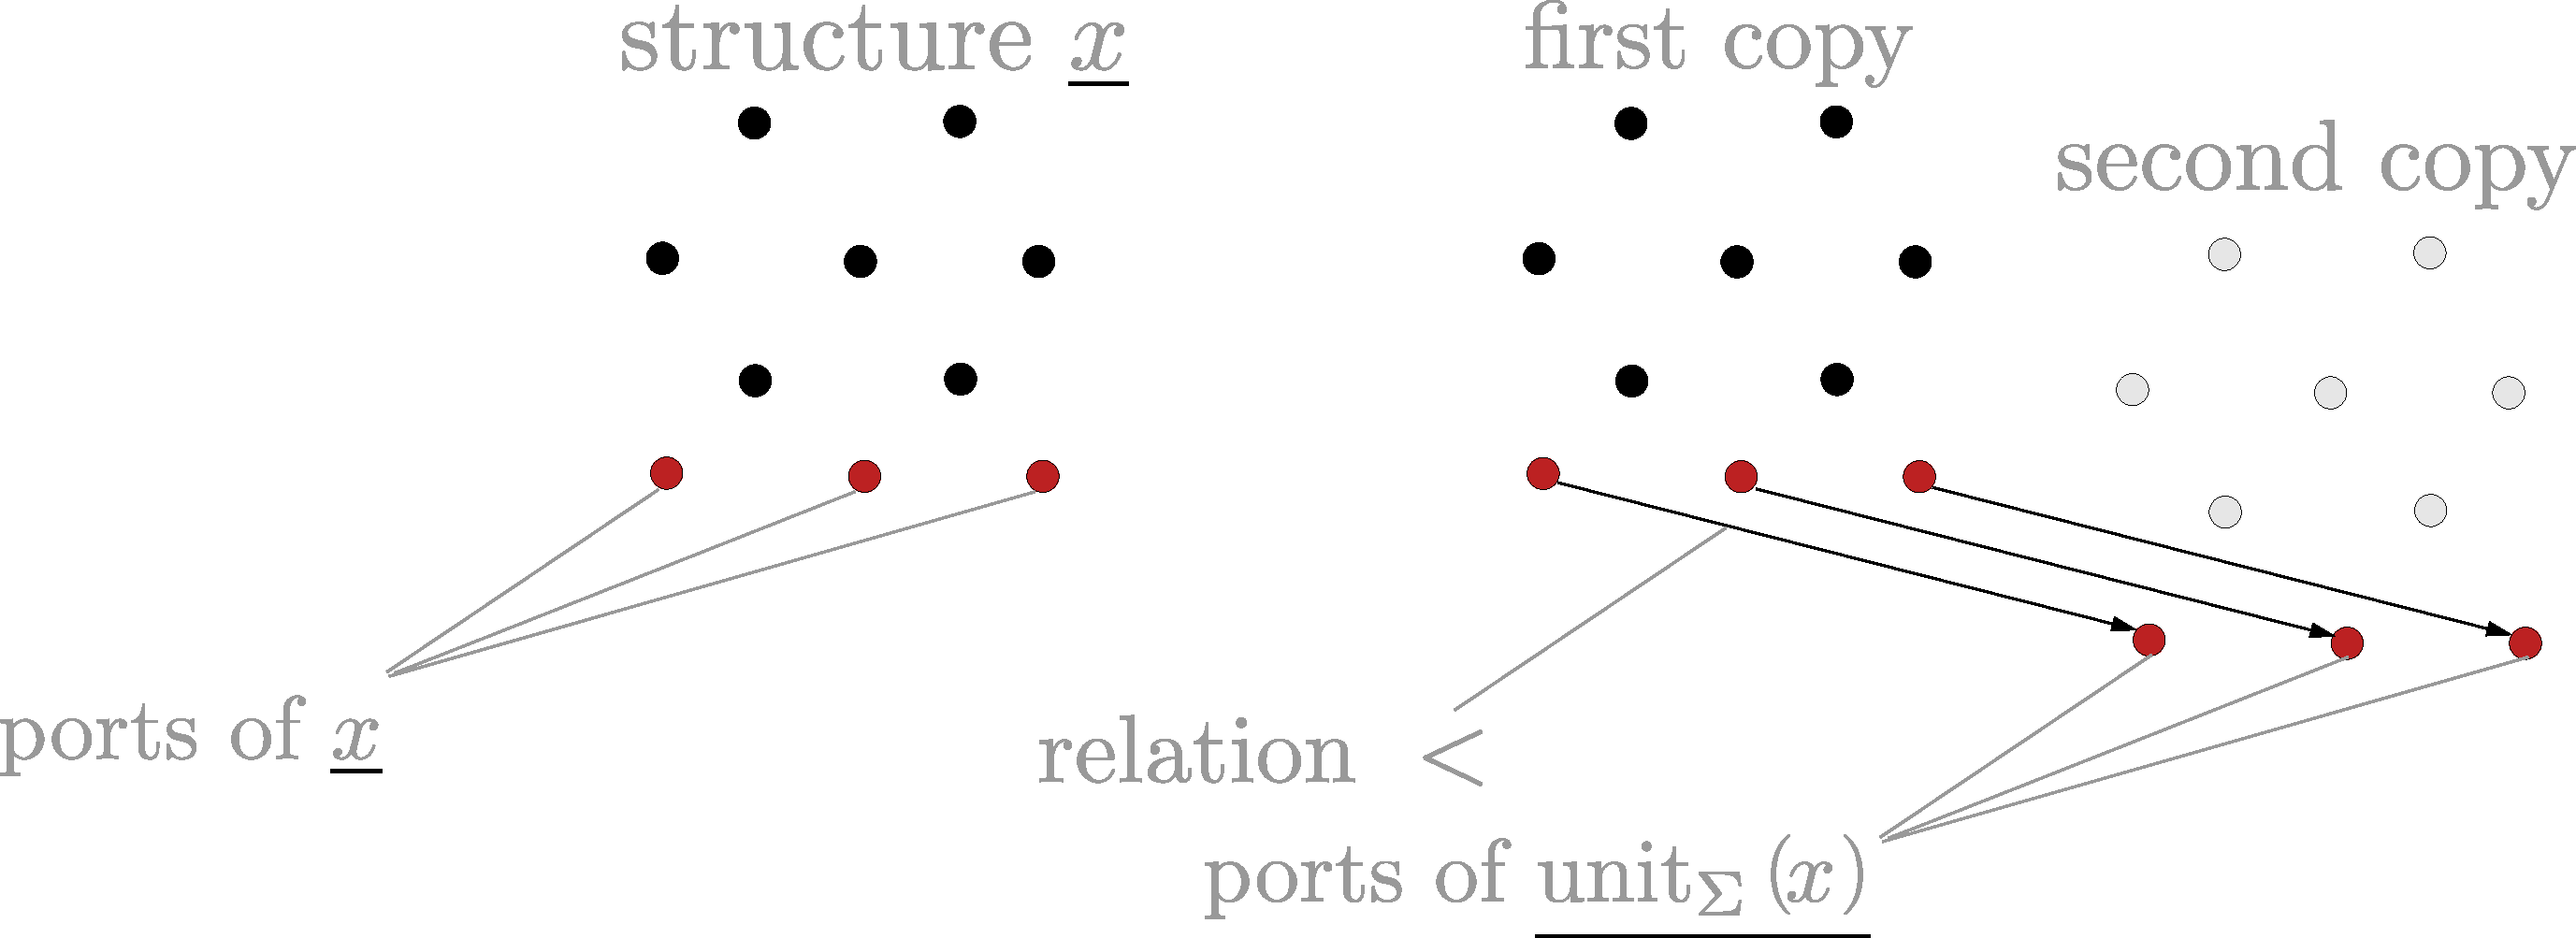
\includegraphics[scale=.18]{pictures/to-logic-unit.pdf}
    \end{center}    
      The universe formulas are then:
    \begin{align*}
    \varphi_1(x)=\mathsf{True} \qquad \varphi_2(x)=\mathsf{Port}_\rSigma(x)
    \end{align*}
    In the first copy, the vocabulary of $\rSigma$ will be interpreted as in the original structure, and as the empty set in the second copy. That is, for every unary relation $R$ and for every binary relation $S$ in the vocabulary of  $\rSigma$, we set:
    \begin{align*}
   \varphi_R^{1}(x)=R(x) \quad&\quad \varphi_S^{1,1}(x,y)=S(x,y)\\
   \varphi_R^{2}(x)=\mathsf{False} \quad&\quad \varphi_S^{2,2}(x,y)=\mathsf{False}
\end{align*}      
Let us interpret the relations $<$ and $\sqsubset$ of the vocabulary of $\tmonad\rSigma$. The  ports of $\underline{\unit(x)}$ inherit the order of the ports of $\underline{x}$, this is why we set:
\begin{align*}
\varphi_\sqsubset^{2,2}(x,y)=x\sqsubset_\rSigma y
\end{align*}
The descendant relation $<$ connects the $i^{th}$ port of $\underline{x}$ to the $i^{th}$ port of $\underline{\unit(x)}$. Since these nodes come from the same node in the original structure, we set:
\begin{align*}
\varphi_<^{1,2}(x,y)=x=y
\end{align*}

\subsubsection{A first-order transduction for monotone unfolding}
\label{sec:fo-transduction-for-unfolding}
Having illustrated the syntax of first-order transduction on the example of the unit function, we describe a first-order transduction for the monotone unfolding operation 
\begin{align*}
    \ranked{\tmonad \mati k{\Sigma} \to \mati k{( \tmonad \Sigma)} + \termset}.
\end{align*}
This is the only prime function whose corresponding first-order transduction is not obvious.
Unlike in Section~\ref{sec:transduction-unit},  we focus more  on the underlying conceptual difficulties than on the syntax of first-order transductions. 

Recall  that when  defining the  monotone  unfolding operation,  for each element $a \in {\tmonad \mati k{\Sigma}}$ of the matrix power, we used a family of (partial) twist functions
\begin{align*}
\to_i : \set{1,\ldots,k} \to \set{1,\ldots,k},
\end{align*}
one for each port $i$ of $a$. For the reader's convenience, we repeat a picture from Section~\ref{sec:unfolding}, which explains the twist functions:
\mypic{109}
In the example  above, the twist functions are:
\begin{align*}
\xymatrix@C=0.5cm@R=1.7cm{
     & && 1 & 2 & 3 \\
    1\ar[urrr]^-{\to_1} & 2 & 3 \ar[urr]^-{\to_1} &&&&
    1\ar[ul]_-{\to_2} & 2\ar[ullll]^-{\to_2} & 3\ar[ulll]_-{\to_2}
}
\end{align*}
In this example, the twist function $\to_1$ is monotone, but  $\to_2$ is not. The monotone unfolding operation works in the same way as general  unfolding, except that it uses the undefined value $\termset$ if the input term has at least one letter which uses at least one non-monotone twist. 

The following lemma, whose simple proof is left to the reader, shows that the twist functions can be defined using first-order logic.
\begin{lemma}
    Let $\rSigma$ be a datatype and let $k \in \set{1,2,\ldots}$. For every partial function
    \begin{align*}
    \tau : \set{1,\ldots,k} \to \set{1,\ldots,k}
    \end{align*}
    there is a first-order formula $\varphi_\tau(x)$ such that for every $a \in \mati k \rSigma$, 
    \begin{align*}
    \underline a \models \varphi_\tau(x)
    \end{align*}
     if and only if $x$ represents a port  with twist function $\tau$.  
\end{lemma}
By using the formulas from the above lemma, one can construct  a first-order formula which checks if a term in $\tmonad \mati k \rSigma$ uses only monotone twists, i.e.~whether or not the output of monotone unfolding should be $\termset$. 

We now proceed to the more interesting part of monotone unfolding, i.e.~actually doing the unfolding for  monotone inputs. Consider an input $t \in \tmonad \mati k \rSigma$ to monotone unfolding.
Define a \emph{sub-node} of $t$ to be a pair (node of $t$, number in $\set{1,\ldots,k$}), as explained in the following picture:
\mypic{124}

In the output of the monotone unfolding, which is of the form
\begin{align*}
(t_1,\ldots,t_k)/f \in \mati k {\tmonad \rSigma},
\end{align*}
the nodes of the  output terms $t_1,\ldots,t_k$ will correspond to the sub-nodes in the input $t$. The sub-nodes can be produced by  copying the input term $k$-times.

The most interesting part of the structure in the output is the descendant relation in the terms $t_1,\ldots,t_k$. This relation  can be viewed as a descendant relation on the sub-nodes. We only describe how the descendant relation on the sub-nodes can be defined in first-order logic, and the rest of the transduction is left to the reader.

When defining the descendant relation on sub-nodes, the crucial part is composing the twist functions.  Suppose that we want to check the descendant relationship between two sub-nodes
\begin{align}\label{eq:descendant-relationship}
(x,i) \stackrel?{\le} (y,j),
\end{align}
where $x,y$ are nodes on the input term and $i,j \in \set{1,\ldots,k}$. We will show that the descendant relationship~\eqref{lem:reduce-descendant-to-ancestor} holds if and only if $x$ is an ancestor of $y$ in the input term,  and the twist functions on the path connecting $x$ and $y$ maps $j$ to $i$, as explained below. 

Consider a path in the input term, which connects  node $x$ with $y$, as  illustrated in the following picture
\mypic{123}    
Each edge in the input term corresponds to a chosen port in some node, which in turn corresponds to some twist function, and therefore it makes sense to talk about the twist function associated to an edge in the input term. Define 
\begin{align*}
\tau_y^x : \set{1,\ldots,k} \to \set{1,\ldots,k}
\end{align*}
to be the partial function, which is obtained by composing all of the twist functions corresponding to edges on the path connecting $y$ to $x$,  starting with $y$ and ending with $x$. In the example from the above picture, we compose two twist functions, which correspond to edges marked in yellow. 

Equipped with the above definitions, we can now characterise the descendant ordering on sub-nodes by
\begin{align*}
    (x,i) \le (y,j) \qquad \text{iff} \qquad x \le y \land \tau_y^x(j)=i.
\end{align*}
Therefore, to complete the proof, it remains to show the following lemma. This is where we use the monotonicity assumption.

\begin{lemma}\label{lem:counter-free}
    For every $i,j \in \set{1,\ldots,k}$ 
    there is a first-order formula $\psi_j^i(x,y)$ such that for every $t  \in \tmonad \mati k \rSigma$
    \begin{align*}
    \underline t \models \psi_j^i(x,y) \qquad \text{iff} \qquad \tau_y^x(j)=i.
    \end{align*}
\end{lemma}
\begin{proof}
    Let $F$ be the set of monotone partial functions  from $\set{1,\ldots,k}$ to itself. Define $L \subseteq F^*$ to be the set of those words $f_1 \cdots f_n$ such that the composition of functions $f_n\circ \cdots \circ f_1$ maps $i$ to $j$. We will show that -- thanks to the monotonicity assumption -- the language is $L$ is definable in first-order logic. By running the corresponding first-order  formula on the path from $x$ to $y$, we get the conclusion of the lemma.   
    
    
    The language $L$ is recognised by a finite automaton, which has states $\set{1,\ldots,k,\bot}$, and which simply applies the function in its input letter to the present state. We show below that this automaton is counter-free, in the sense of McNaughton and Papert~\cite[p.~6]{McNaughtonPapert71}, and therefore it can be defined in first-order logic. 

    Recall that a counter in an automaton is a sequence of at least two pairwise distinct states $q_1,\ldots,q_n$ such that
    \begin{align*}
    q_1  \stackrel w \to q_2 \stackrel w \to \cdots \stackrel w \to q_n \stackrel w \to q_1
    \end{align*}
    holds for some common input string $w$. In the automaton for the language $L$ that we have discussed above, there is no counter. Indeed, if we would have $q_1 \le q_2$, then by monotonicity of the function   $w \in F$ we would have 
    \begin{align*}
    q_1 \le q_2 \le \cdots \le q_n \le q_1
    \end{align*}
    and therefore all of $q_1,\ldots,q_n$ would be equal, contradicting the assumption that they are pairwise distinct. The same argument would work when $q_1 \ge q_2$. By~\cite[Theorem 10.5]{McNaughtonPapert71}, if an automaton has no counter, then its language is definable in first-order logic. 
    
\end{proof}